%TODO Remind Peter that ɔ has a problem of typesetting, I don't see it.


%\documentclass[output=paper]{LSP/langsci} 
%\author{??? Bennett\affiliation{???}} 
%\begin{styleHeading}
\documentclass[output=paper
,newtxmath
,modfonts
,nonflat]{langsci/langscibook}
% \usepackage{pifont}
\usepackage{savesym}

\savesymbol{downingtriple}
\savesymbol{downingdouble}
\savesymbol{downingquad}
\savesymbol{downingquint}
\savesymbol{suph}
\savesymbol{supj}
\savesymbol{supw}
\savesymbol{sups}
\savesymbol{ts}
\savesymbol{tS}
\savesymbol{devi}
\savesymbol{devu}
\savesymbol{devy}
\savesymbol{deva}
\savesymbol{N}
\savesymbol{Z}
\savesymbol{circled}
\savesymbol{sem}
\savesymbol{row}
\savesymbol{tipa}
\savesymbol{tableauxcounter}
\savesymbol{tabhead}
\savesymbol{inp}
\savesymbol{inpno}
\savesymbol{g}
\savesymbol{hanl}
\savesymbol{hanr}
\savesymbol{kuku}
\savesymbol{ip}
\savesymbol{lipm}
\savesymbol{ripm}
\savesymbol{lipn}
\savesymbol{ripn} 
% \usepackage{amsmath} 
% \usepackage{multicol}
\usepackage{qtree} 
\usepackage{tikz-qtree,tikz-qtree-compat}
% \usepackage{tikz}
\usepackage{upgreek}


%%%%%%%%%%%%%%%%%%%%%%%%%%%%%%%%%%%%%%%%%%%%%%%%%%%%
%%%                                              %%%
%%%           Examples                           %%%
%%%                                              %%%
%%%%%%%%%%%%%%%%%%%%%%%%%%%%%%%%%%%%%%%%%%%%%%%%%%%%
% remove the percentage signs in the following lines
% if your book makes use of linguistic examples
\usepackage{tipa}  
\usepackage{pstricks,pst-xkey,pst-asr}

%for sande et al
\usepackage{pst-jtree}
\usepackage{pst-node}
%\usepackage{savesym}


% \usepackage{subcaption}
\usepackage{multirow}  
\usepackage{./langsci/styles/langsci-optional} 
\usepackage{./langsci/styles/langsci-lgr} 
\usepackage{./langsci/styles/langsci-glyphs} 
\usepackage[normalem]{ulem}
%% if you want the source line of examples to be in italics, uncomment the following line
% \def\exfont{\it}
\usetikzlibrary{arrows.meta,topaths,trees}
\usepackage[linguistics]{forest}
\forestset{
	fairly nice empty nodes/.style={
		delay={where content={}{shape=coordinate,for parent={
					for children={anchor=north}}}{}}
}}
\usepackage{soul}
\usepackage{arydshln}
% \usepackage{subfloat}
\usepackage{langsci/styles/langsci-gb4e} 
   
% \usepackage{linguex}
\usepackage{vowel}

\usepackage{pifont}% http://ctan.org/pkg/pifont
\newcommand{\cmark}{\ding{51}}%
\newcommand{\xmark}{\ding{55}}%
 
 
 %Lamont
 \makeatletter
\g@addto@macro\@floatboxreset\centering
\makeatother

\usepackage{newfloat} 
\DeclareFloatingEnvironment[fileext=tbx,name=Tableau]{tableau}
% %% hyphenation points for line breaks
%% Normally, automatic hyphenation in LaTeX is very good
%% If a word is mis-hyphenated, add it to this file
%%
%% add information to TeX file before \begin{document} with:
%% %% hyphenation points for line breaks
%% Normally, automatic hyphenation in LaTeX is very good
%% If a word is mis-hyphenated, add it to this file
%%
%% add information to TeX file before \begin{document} with:
%% %% hyphenation points for line breaks
%% Normally, automatic hyphenation in LaTeX is very good
%% If a word is mis-hyphenated, add it to this file
%%
%% add information to TeX file before \begin{document} with:
%% \include{localhyphenation}
\hyphenation{
affri-ca-te
affri-ca-tes
com-ple-ments
par-a-digm
Sha-ron
Kings-ton
phe-nom-e-non
Daul-ton
Abu-ba-ka-ri
Ngo-nya-ni
Clem-ents 
King-ston
Tru-cken-brodt
Tab-leau
cophono-logies
mark-edness
Ti-gri-nya
a-mong
Car-stens
Lu-bu-ku-su
}
\hyphenation{
affri-ca-te
affri-ca-tes
com-ple-ments
par-a-digm
Sha-ron
Kings-ton
phe-nom-e-non
Daul-ton
Abu-ba-ka-ri
Ngo-nya-ni
Clem-ents 
King-ston
Tru-cken-brodt
Tab-leau
cophono-logies
mark-edness
Ti-gri-nya
a-mong
Car-stens
Lu-bu-ku-su
}
\hyphenation{
affri-ca-te
affri-ca-tes
com-ple-ments
par-a-digm
Sha-ron
Kings-ton
phe-nom-e-non
Daul-ton
Abu-ba-ka-ri
Ngo-nya-ni
Clem-ents 
King-ston
Tru-cken-brodt
Tab-leau
cophono-logies
mark-edness
Ti-gri-nya
a-mong
Car-stens
Lu-bu-ku-su
}
% %add all your local new commands to this file
\newcommand{\downingquad}[4]{\parbox{2.5cm}{#1}\parbox{3.5cm}{#2}\parbox{2.5cm}{#3}\parbox{3.5cm}{#4}}
\newcommand{\downingtriple}[3]{\parbox{4.5cm}{#1}\parbox{3cm}{#2}\parbox{3cm}{#3}}
\newcommand{\downingdouble}[2]{\parbox{4.5cm}{#1}\parbox{6cm}{#2}}
\newcommand{\downingquint}[5]{\parbox{1.75cm}{#1}\parbox{2.25cm}{#2}\parbox{2cm}{#3}\parbox{3cm}{#4}\parbox{2cm}{#5}}
\newcolumntype{Y}{>{\centering\arraybackslash}X}
\newcolumntype{T}{>{\centering\arraybackslash}m{2cm}}

%commands for Kusmer paper below
\newcommand{\ip}{$\upiota$}
\newcommand{\lipm}{(\_{\ip-Max}}
\newcommand{\ripm}{)\_{\ip-Max}}
\newcommand{\lipn}{(\_{\ip}}
\newcommand{\ripn}{)\_{\ip}}
\renewcommand{\_}[1]{\textsubscript{#1}}


%commands for Pillion paper below
\newcommand{\suph}{\textipa{\super h}}
\newcommand{\supj}{\textipa{\super j}}
\newcommand{\supw}{\textipa{\super w}}
\newcommand{\ts}{\textipa{\t{ts}}}
\newcommand{\tS}{\textipa{\t{tS}}}
\newcommand{\devi}{\textipa{\r*i}}
\newcommand{\devu}{\textipa{\r*u}}
\newcommand{\devy}{\textipa{\r*y}}
\newcommand{\deva}{\textipa{\r*a}}
\renewcommand{\N}{\textipa{N}}
\newcommand{\Z}{\textipa{Z}}
% 

%commands for Diercks paper below
\newcommand{\circled}[1]{\begin{tikzpicture}[baseline=(word.base)]
\node[draw, rounded corners, text height=8pt, text depth=2pt, inner sep=2pt, outer sep=0pt, use as bounding box] (word) {#1};
\end{tikzpicture}
}

%commands for Pesetsky paper below
% \newcommand{\sem}[2][]{\mbox{$[\![ $\textbf{#2}$ ]\!]^{#1}$}}
\newcommand{\sem}[2][]{\mbox{$[[ $\textbf{#2}$ ]]^{#1}$}}

% \newcommand{\ripn}{{\color{red}ripn}}%this is used but never defined. Please update the definition



%commands for Lamont paper below
\newcommand{\row}[4]{
	#1. & 
    /{#2}/ & 
    [{#3}] & 
    `#4' \\ 
}
%\newcounter{tableauxcounter}
\newcommand{\tabhead}[2]{
%     \captionsetup{labelformat=empty}
%     \stepcounter{tableauxcounter}
%     \addtocounter{table}{-1}
% 	\centering
% 	\caption{Tableau \thetableauxcounter: #1}
	\caption{#1}
	\label{#2}
}
\newcommand{\candref}[2]{{(\ref{#1}#2)}}
\newcommand{\tableauref}[1]{{Tableau~\ref{#1}}}
% tableaux
\newcommand{\inp}[1]{\multicolumn{2}{|l||}{{#1}}}
\newcommand{\inpno}[1]{\multicolumn{2}{|l||}{#1}}
\newcommand{\g}{\cellcolor{lightgray}}
\newcommand{\hanl}{\HandLeft}
\newcommand{\hanr}{\HandRight}
\newcommand{\kuku}{Kuk\'{u}}

% \newcommand{\nocaption}[1]{{\color{red} Please provide a caption}}

% \providecommand{\biberror}[1]{{\color{red}#1}}

\definecolor{RED}{cmyk}{0.05,1,0.8,0}


\newfontfamily\amharicfont[Script = Ethiopic, Scale = 1.0]{AbyssinicaSIL}
\newcommand{\amh}[1]{{\amharicfont #1}}

% 
% %Gjersoe
\usepackage{textgreek}
% 
\newcommand{\viol}{\fontfamily{MinionPro-OsF}\selectfont\rotatebox{60}{$\star$}}
\newcommand{\myscalex}{0.45}
\newcommand{\myscaley}{0.65}
%\newcommand{\red}[1]{\textcolor{red}{#1}}
%\newcommand{\blue}[1]{\textcolor{blue}{#1}}
\newcommand{\epen}[1]{\colorbox{jgray}{#1}}
\newcommand{\hand}{{\normalsize \ding{43}}}
\definecolor{jgray}{gray}{0.8} 
\usetikzlibrary{positioning}
\usetikzlibrary{matrix}
\newcommand{\mora}{\textmu\xspace}
\newcommand{\si}{\textsigma\xspace}
\newcommand{\ft}{\textPhi\xspace}
\newcommand{\tone}{\texttau\xspace}
\newcommand{\word}{\textomega\xspace}
% \newcommand{\ts}{\texttslig}
\newcommand{\fns}{\footnotesize}
\newcommand{\ns}{\normalsize}
\newcommand{\vs}{\vspace{1em}}
\newcommand{\bs}{\textbackslash}   % backslash
\newcommand{\cmd}[1]{{\bf \color{red}#1}}   % highlights command
\newcommand{\scell}[2][l]{\begin{tabular}[#1]{@{}c@{}}#2\end{tabular}}
% \interfootnotelinepenalty=10000

% --- Snider Representations --- %

\newcommand{\RepLevelHh}{
\begin{minipage}{0.10\textwidth}
\begin{tikzpicture}[xscale=\myscalex,yscale=\myscaley]
%\node (syl) at (0,0) {Hi};
\node (Rt) at (0,1) {o};
\node (H) at (-0.5,2) {H};
\node (R) at (0.5,3) {h};
%\draw [thick] (syl.north) -- (Rt.south) ;
\draw [thick] (Rt.north) -- (H.south) ;
\draw [thick] (Rt.north) -- (R.south) ;
\end{tikzpicture}
\end{minipage}
}

\newcommand{\RepLevelLh}{
\begin{minipage}{0.10\textwidth}
\begin{tikzpicture}[xscale=\myscalex,yscale=\myscaley]
%\node (syl) at (0,0) {Mid2};
\node (Rt) at (0,1) {o};
\node (H) at (-0.5,2) {L};
\node (R) at (0.5,3) {h};
%\draw [thick] (syl.north) -- (Rt.south) ;
\draw [thick] (Rt.north) -- (H.south) ;
\draw [thick] (Rt.north) -- (R.south) ;
\end{tikzpicture}
\end{minipage}
}

\newcommand{\RepLevelHl}{
\begin{minipage}{0.10\textwidth}
\begin{tikzpicture}[xscale=\myscalex,yscale=\myscaley]
%\node (syl) at (0,0) {Mid1};
\node (Rt) at (0,1) {o};
\node (H) at (-0.5,2) {H};
\node (R) at (0.5,3) {l};
%\draw [thick] (syl.north) -- (Rt.south) ;
\draw [thick] (Rt.north) -- (H.south) ;
\draw [thick] (Rt.north) -- (R.south) ;
\end{tikzpicture}
\end{minipage}
}

\newcommand{\RepLevelLl}{
\begin{minipage}{0.10\textwidth}
\begin{tikzpicture}[xscale=\myscalex,yscale=\myscaley]
%\node (syl) at (0,0) {Lo};
\node (Rt) at (0,1) {o};
\node (H) at (-0.5,2) {L};
\node (R) at (0.5,3) {l};
%\draw [thick] (syl.north) -- (Rt.south) ;
\draw [thick] (Rt.north) -- (H.south) ;
\draw [thick] (Rt.north) -- (R.south) ;
\end{tikzpicture}
\end{minipage}
}

% --- Representations --- %

\newcommand{\RepLevel}{
\begin{minipage}{0.10\textwidth}
\begin{tikzpicture}[xscale=\myscalex,yscale=\myscaley]
\node (syl) at (0,0) {\textsigma};
\node (Rt) at (0,1) {o};
\node (H) at (-0.5,2) {\texttau};
\node (R) at (0.5,3) {\textrho};
\draw [thick] (syl.north) -- (Rt.south) ;
\draw [thick] (Rt.north) -- (H.south) ;
\draw [thick] (Rt.north) -- (R.south) ;
\end{tikzpicture}
\end{minipage}
}

\newcommand{\RepContour}{
\begin{minipage}{0.10\textwidth}
\begin{tikzpicture}[xscale=\myscalex,yscale=\myscaley]
\node (syl) at (0,0) {\textsigma};
\node (Rt) at (0,1) {o};
\node (H) at (-0.5,2) {\texttau};
\node (R) at (0.5,3) {\textrho};
\node (Rt2) at (1.5,1.0) {o};
%\node (H2) at (1.0,2) {$\tau$};
%\node (R2) at (2.0,2.5) {R};
\draw [thick] (syl.north) -- (Rt.south) ;
\draw [thick] (Rt.north) -- (H.south) ;
\draw [thick] (Rt.north) -- (R.south) ;
\draw [thick] (syl.north) -- (Rt2.south) ;
%\draw [thick] (Rt2.north) -- (H2.south) ;
%\draw [thick] (Rt2.north) -- (R2.south) ;
\end{tikzpicture}
\end{minipage}
}


% --- OT constraints --- %

\newcommand{\IllustrationDown}{
\begin{minipage}{0.09\textwidth}
\begin{tikzpicture}[xscale=0.7,yscale=0.45]
\node (reg) at (0,0.75) {{\small \textalpha}};
\node (arrow) at (0,0) {{\fns $\downarrow$}};
\node (Rt) at (0,-0.75) {{\small \textbeta}};
\end{tikzpicture}
\end{minipage}
}

\newcommand{\IllustrationUp}{
\begin{minipage}{0.09\textwidth}
\begin{tikzpicture}[xscale=0.7,yscale=0.45]
\node (reg) at (0,0.75) {{\small \textalpha}};
\node (arrow) at (0,0) {{\fns $\uparrow$}};
\node (Rt) at (0,-0.75) {{\small \textbeta}};
\end{tikzpicture}
\end{minipage}
}

\newcommand{\MaxAB}{
\begin{minipage}{0.09\textwidth}
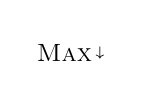
\begin{tikzpicture}[xscale=0.6,yscale=0.4]
\node (max) at (0,0) {{\small \textsc{Max}}};
\node (reg) at (0.75,0.5) {{\fns \textalpha}};
\node (arrow) at (0.75,0) {{\tiny $\downarrow$}};
\node (Rt) at (0.75,-0.5) {{\fns \textbeta}};
\end{tikzpicture}
\end{minipage}
}

\newcommand{\DepAB}{
\begin{minipage}{0.09\textwidth}
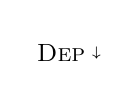
\begin{tikzpicture}[xscale=0.6,yscale=0.4]
\node (max) at (0,0) {{\small \textsc{Dep}}};
\node (reg) at (0.75,0.5) {{\fns \textalpha}};
\node (arrow) at (0.75,0) {{\tiny $\downarrow$}};
\node (Rt) at (0.75,-0.5) {{\fns \textbeta}};
\end{tikzpicture}
\end{minipage}
}

\newcommand{\DepHReg}{
\begin{minipage}{0.055\textwidth}
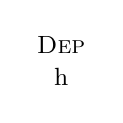
\begin{tikzpicture}[xscale=0.6,yscale=0.4]
\node (dep) at (0,0) {{\small \textsc{Dep}}};
\node (reg) at (0,-1.0) {{\small h}};
\end{tikzpicture}
\end{minipage}
}

\newcommand{\DepLReg}{
\begin{minipage}{0.055\textwidth}
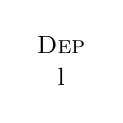
\begin{tikzpicture}[xscale=0.6,yscale=0.4]
\node (dep) at (0,0) {{\small \textsc{Dep}}};
\node (reg) at (0,-1.0) {{\small l}};
\end{tikzpicture}
\end{minipage}
}

\newcommand{\DepReg}{
\begin{minipage}{0.055\textwidth}
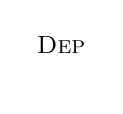
\begin{tikzpicture}[xscale=0.6,yscale=0.4]
\node (dep) at (0,0) {{\small \textsc{Dep}}};
\node (reg) at (0,-1.0) {{\small \textrho}};
\end{tikzpicture}
\end{minipage}
}

\newcommand{\DepTRt}{
\begin{minipage}{0.1\textwidth}
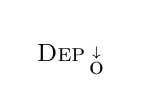
\begin{tikzpicture}[xscale=0.6,yscale=0.4]
\node (dep) at (0,0) {{\small \textsc{Dep}}};
\node (t) at (0.75,0.5) {{\fns \texttau}};
\node (arrow) at (0.75,0) {{\tiny $\downarrow$}};
\node (Rt) at (0.75,-0.5) {{\fns o}};
\end{tikzpicture}
\end{minipage}
}

\newcommand{\MaxRegRt}{
\begin{minipage}{0.1\textwidth}
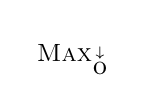
\begin{tikzpicture}[xscale=0.6,yscale=0.4]
\node (max) at (0,0) {{\small \textsc{Max}}};
\node (arrow) at (0.75,0) {{\tiny $\downarrow$}};
\node (Rt) at (0.75,-0.5) {{\fns o}};
\node (reg) at (0.75,0.5) {{\fns \textrho}};
\end{tikzpicture}
\end{minipage}
}

\newcommand{\RegToneByRt}{
\begin{minipage}{0.06\textwidth}
\begin{tikzpicture}[xscale=0.6,yscale=0.5]
\node[rotate=20] (arrow1) at (-0.15,0) {{\fns $\uparrow$}};
\node[rotate=340] (arrow2) at (0.15,0) {{\fns $\uparrow$}};
\node (Rt) at (0,-0.55) {{\small o}};
\node (reg) at (0.4,0.55) {{\small \textrho}};
\node (tone) at (-0.4,0.55) {{\small \texttau}};
\end{tikzpicture}
\end{minipage}
}

\newcommand{\RegToneBySyl}{
\begin{minipage}{0.06\textwidth}
\begin{tikzpicture}[xscale=0.6,yscale=0.5]
\node[rotate=20] (arrow1) at (-0.15,0) {{\fns $\uparrow$}};
\node[rotate=340] (arrow2) at (0.15,0) {{\fns $\uparrow$}};
\node (Rt) at (0,-0.55) {{\small \textsigma}};
\node (reg) at (0.4,0.55) {{\small \textrho}};
\node (tone) at (-0.4,0.55) {{\small \texttau}};
\end{tikzpicture}
\end{minipage}
}

\newcommand{\DepTone}{
\begin{minipage}{0.055\textwidth}
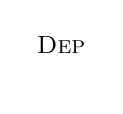
\begin{tikzpicture}[xscale=0.6,yscale=0.4]
\node (dep) at (0,0) {{\small \textsc{Dep}}};
\node (tone) at (0,-1.0) {{\small \texttau}};
\end{tikzpicture}
\end{minipage}
}

\newcommand{\DepTonalRt}{
\begin{minipage}{0.055\textwidth}
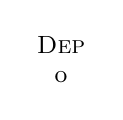
\begin{tikzpicture}[xscale=0.6,yscale=0.4]
\node (dep) at (0,0) {{\small \textsc{Dep}}};
\node (tone) at (0,-1.0) {{\small o}};
\end{tikzpicture}
\end{minipage}
}

\newcommand{\DepL}{
\begin{minipage}{0.055\textwidth}
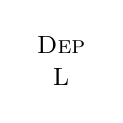
\begin{tikzpicture}[xscale=0.6,yscale=0.4]
\node (dep) at (0,0) {{\small \textsc{Dep}}};
\node (tone) at (0,-1.0) {{\small L}};
\end{tikzpicture}
\end{minipage}
}

\newcommand{\DepH}{
\begin{minipage}{0.055\textwidth}
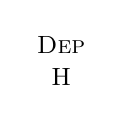
\begin{tikzpicture}[xscale=0.6,yscale=0.4]
\node (dep) at (0,0) {{\small \textsc{Dep}}};
\node (tone) at (0,-1.0) {{\small H}};
\end{tikzpicture}
\end{minipage}
}

\newcommand{\NoMultDiff}{{\small *loh}}
\newcommand{\Alt}{{\small \textsc{Alt}}}
\newcommand{\NoSkip}{{\small \scell{\textsc{No}\\\textsc{Skip}}}}


\newcommand{\RegDomRt}{
\begin{minipage}{0.030\textwidth}
\begin{tikzpicture}[xscale=0.6,yscale=0.5]
\node (arrow) at (0,0) {{\fns $\downarrow$}};
\node (Rt) at (0,-0.55) {{\small o}};
\node (reg) at (0,0.55) {{\small \textrho}};
\end{tikzpicture}
\end{minipage}
}

\newcommand{\DepRegRt}{
\begin{minipage}{0.1\textwidth}
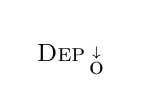
\begin{tikzpicture}[xscale=0.6,yscale=0.4]
\node (dep) at (0,0) {{\small \textsc{Dep}}};
\node (arrow) at (0.75,0) {{\tiny $\downarrow$}};
\node (Rt) at (0.75,-0.5) {{\fns o}};
\node (reg) at (0.75,0.5) {{\fns \textrho}};
\end{tikzpicture}
\end{minipage}
}

% unused

\newcommand{\ToneByRt}{
\begin{minipage}{0.05\textwidth}
\begin{tikzpicture}[xscale=0.6,yscale=0.5]
\node (arrow) at (0,0) {{\fns $\uparrow$}};
\node (Rt) at (0,-0.55) {{\small o}};
\node (tone) at (0,0.55) {{\small \texttau}};
\end{tikzpicture}
\end{minipage}
}

\newcommand{\RegByRt}{
\begin{minipage}{0.05\textwidth}
\begin{tikzpicture}[xscale=0.6,yscale=0.5]
\node (arrow) at (0,0) {{\fns $\uparrow$}};
\node (Rt) at (0,-0.55) {{\small o}};
\node (reg) at (0,0.55) {{\small \textrho}};
\end{tikzpicture}
\end{minipage}
}

\newcommand{\ToneDomRt}{
\begin{minipage}{0.05\textwidth}
\begin{tikzpicture}[xscale=0.6,yscale=0.5]
\node (arrow) at (0,0) {{\fns $\downarrow$}};
\node (Rt) at (0,-0.55) {{\small o}};
\node (tone) at (0,0.55) {{\small \texttau}};
\end{tikzpicture}
\end{minipage}
}

% --- OT tableaus --- %

% Sec. 3.2, first tabl.

\newcommand{\OTHLInput}{
\begin{minipage}{0.17\textwidth}
\begin{tikzpicture}[xscale=\myscalex,yscale=\myscaley]
\node (tone) at (2,0) {(= H)};
\node (syl) at (0,0) {\textsigma};
\node (Rt) at (0,1) {o};
\node (H) at (-0.5,2) {H};
\node (R) at (0.5,3) {h};
\node (Rt2) at (1.5,1.0) {o};
%\node (H2) at (1.0,2) {\epen{L}};
\node (R2) at (2.0,3) {\blue{l}};
\draw [thick] (syl.north) -- (Rt.south) ;
\draw [thick] (Rt.north) -- (H.south) ;
\draw [thick] (Rt.north) -- (R.south) ;
\draw [thick] (syl.north) -- (Rt2.south) ;
%\draw [dashed] (Rt2.north) -- (H2.south) ;
%\draw [dashed] (Rt2.north) -- (R2.south) ;
\end{tikzpicture}
\end{minipage}
}

\newcommand{\OTHLWinner}{
\begin{minipage}{0.17\textwidth}
\begin{tikzpicture}[xscale=\myscalex,yscale=\myscaley]
\node (tone) at (2,0) {(= HL)};
\node (syl) at (0,0) {\textsigma};
\node (Rt) at (0,1) {o};
\node (H) at (-0.5,2) {H};
\node (R) at (0.5,3) {h};
\node (Rt2) at (1.5,1.0) {o};
\node (H2) at (1.0,2) {\epen{L}};
\node (R2) at (2.0,3) {\blue{l}};
\draw [thick] (syl.north) -- (Rt.south) ;
\draw [thick] (Rt.north) -- (H.south) ;
\draw [thick] (Rt.north) -- (R.south) ;
\draw [thick] (syl.north) -- (Rt2.south) ;
\draw [dashed] (Rt2.north) -- (H2.south) ;
\draw [dashed] (Rt2.north) -- (R2.south) ;
\end{tikzpicture}
\end{minipage}
}

\newcommand{\OTHLSpreadingHOnly}{
\begin{minipage}{0.17\textwidth}
\begin{tikzpicture}[xscale=\myscalex,yscale=\myscaley]
\node (tone) at (2,0) {(= HM)};
\node (syl) at (0,0) {\textsigma};
\node (Rt) at (0,1) {o};
\node (H) at (-0.5,2) {H};
\node (R) at (0.5,3) {h};
\node (Rt2) at (1.5,1.0) {o};
%\node (H2) at (1.0,2) {\epen{L}};
\node (R2) at (2.0,3) {\blue{l}};
\draw [thick] (syl.north) -- (Rt.south) ;
\draw [thick] (Rt.north) -- (H.south) ;
\draw [thick] (Rt.north) -- (R.south) ;
\draw [thick] (syl.north) -- (Rt2.south) ;
\draw [dashed] (Rt2.north) -- (R2.south) ;
\draw [dashed] (Rt2.north) -- (H.south) ;
\end{tikzpicture}
\end{minipage}
}

\newcommand{\OTHLInsertH}{
\begin{minipage}{0.17\textwidth}
\begin{tikzpicture}[xscale=\myscalex,yscale=\myscaley]
\node (tone) at (2,0) {(= HM)};
\node (syl) at (0,0) {\textsigma};
\node (Rt) at (0,1) {o};
\node (H) at (-0.5,2) {H};
\node (R) at (0.5,3) {h};
\node (Rt2) at (1.5,1.0) {o};
\node (H2) at (1.0,2) {\epen{H}};
\node (R2) at (2.0,3) {\blue{l}};
\draw [thick] (syl.north) -- (Rt.south) ;
\draw [thick] (Rt.north) -- (H.south) ;
\draw [thick] (Rt.north) -- (R.south) ;
\draw [thick] (syl.north) -- (Rt2.south) ;
\draw [dashed] (Rt2.north) -- (H2.south) ;
\draw [dashed] (Rt2.north) -- (R2.south) ;
\end{tikzpicture}
\end{minipage}
}

\newcommand{\OTHLOverwriting}{
\begin{minipage}{0.17\textwidth}
\begin{tikzpicture}[xscale=\myscalex,yscale=\myscaley]
\node (syl) at (0,0) {\textsigma};
\node (Rt) at (0,1) {o};
\node (H) at (-0.5,2) {H};
\node (R) at (0.5,3) {h};
\node (Rt2) at (1.5,1.0) {o};
%\node (H2) at (1.0,2) {\epen{L}};
\node (R2) at (2.0,3) {\blue{l}};
\draw [thick] (syl.north) -- (Rt.south) ;
\draw [thick] (Rt.north) -- (H.south) ;
\draw [thick] (Rt.north) -- (R.south) ;
\draw [thick] (syl.north) -- (Rt2.south) ;
%\draw [dashed] (Rt2.north) -- (H2.south) ;
\draw [dashed] (Rt.north) -- (R2.south) ;
\node (del) at (0.3,1.9) {\textbf{=}};
\end{tikzpicture}
\end{minipage}
}

\newcommand{\OTHLSpreading}{
\begin{minipage}{0.17\textwidth}
\begin{tikzpicture}[xscale=\myscalex,yscale=\myscaley]
\node (syl) at (0,0) {\textsigma};
\node (Rt) at (0,1) {o};
\node (H) at (-0.5,2) {H};
\node (R) at (0.5,3) {h};
\node (Rt2) at (1.5,1.0) {o};
%\node (H2) at (1.0,2) {\epen{L}};
\node (R2) at (2.0,3) {\blue{l}};
\draw [thick] (syl.north) -- (Rt.south) ;
\draw [thick] (Rt.north) -- (H.south) ;
\draw [thick] (Rt.north) -- (R.south) ;
\draw [thick] (syl.north) -- (Rt2.south) ;
%\draw [dashed] (Rt2.north) -- (H2.south) ;
\draw [dashed] (Rt2.north) -- (H.south) ;
\draw [dashed] (Rt2.north) -- (R.south) ;
\end{tikzpicture}
\end{minipage}
}

% Sec. 4.2, second tabl.: phrase-medial position

\newcommand{\OTHnoLInput}{
\begin{minipage}{0.17\textwidth}
\begin{tikzpicture}[xscale=\myscalex,yscale=\myscaley]
\node (tone) at (2,0) {(= H)};
\node (syl) at (0,0) {\textsigma};
\node (Rt) at (0,1) {o};
\node (H) at (-0.5,2) {H};
\node (R) at (0.5,3) {h};
\node (Rt2) at (1.5,1.0) {o};
%\node (H2) at (1.0,2) {\epen{L}};
%\node (R2) at (2.0,3) {\blue{l}};
\draw [thick] (syl.north) -- (Rt.south) ;
\draw [thick] (Rt.north) -- (H.south) ;
\draw [thick] (Rt.north) -- (R.south) ;
\draw [thick] (syl.north) -- (Rt2.south) ;
\end{tikzpicture}
\end{minipage}
}

\newcommand{\OTHnoLEpenth}{
\begin{minipage}{0.17\textwidth}
\begin{tikzpicture}[xscale=\myscalex,yscale=\myscaley]
\node (tone) at (2,0) {(= HM)};
\node (syl) at (0,0) {\textsigma};
\node (Rt) at (0,1) {o};
\node (H) at (-0.5,2) {H};
\node (R) at (0.5,3) {h};
\node (Rt2) at (1.5,1.0) {o};
\node (H2) at (1.0,2) {\epen{L}};
\node (R2) at (2.0,3) {\epen{h}};
\draw [thick] (syl.north) -- (Rt.south) ;
\draw [thick] (Rt.north) -- (H.south) ;
\draw [thick] (Rt.north) -- (R.south) ;
\draw [thick] (syl.north) -- (Rt2.south) ;
\draw [dashed] (Rt2.north) -- (H2.south) ;
\draw [dashed] (Rt2.north) -- (R2.south) ;
\end{tikzpicture}
\end{minipage}
}

\newcommand{\OTHnoLSpreading}{
\begin{minipage}{0.17\textwidth}
\begin{tikzpicture}[xscale=\myscalex,yscale=\myscaley]
\node (tone) at (2,0) {(= HH)};
\node (syl) at (0,0) {\textsigma};
\node (Rt) at (0,1) {o};
\node (H) at (-0.5,2) {H};
\node (R) at (0.5,3) {h};
\node (Rt2) at (1.5,1.0) {o};
%\node (H2) at (1.0,2) {\epen{L}};
%\node (R2) at (2.0,3) {\blue{l}};
\draw [thick] (syl.north) -- (Rt.south) ;
\draw [thick] (Rt.north) -- (H.south) ;
\draw [thick] (Rt.north) -- (R.south) ;
\draw [thick] (syl.north) -- (Rt2.south) ;
\draw [dashed] (Rt2.north) -- (H.south) ;
\draw [dashed] (Rt2.north) -- (R.south) ;
\end{tikzpicture}
\end{minipage}
}

% Sec. 4.2, third tabl., LM is unaffected by L\%

\newcommand{\OTLMInput}{
\begin{minipage}{0.2\textwidth}
\begin{tikzpicture}[xscale=\myscalex,yscale=\myscaley]
\node (tone) at (2,0) {(= LM)};
\node (syl) at (0,0) {\textsigma};
\node (Rt) at (0,1) {o};
\node (H) at (-0.5,2) {L};
\node (R) at (0.5,3) {l};
\node (Rt2) at (1.5,1.0) {o};
\node (H2) at (1.0,2) {L};
\node (R2) at (2.0,3) {h};
\node (R3) at (3.0,3) {\blue{l}};
\draw [thick] (syl.north) -- (Rt.south) ;
\draw [thick] (Rt.north) -- (H.south) ;
\draw [thick] (Rt.north) -- (R.south) ;
\draw [thick] (syl.north) -- (Rt2.south) ;
\draw [thick] (Rt2.north) -- (H2.south) ;
\draw [thick] (Rt2.north) -- (R2.south) ;
\end{tikzpicture}
\end{minipage}
}

\newcommand{\OTLMReplace}{
\begin{minipage}{0.2\textwidth}
\begin{tikzpicture}[xscale=\myscalex,yscale=\myscaley]
\node (tone) at (2,0) {(= LL)};
\node (syl) at (0,0) {\textsigma};
\node (Rt) at (0,1) {o};
\node (H) at (-0.5,2) {L};
\node (R) at (0.5,3) {l};
\node (Rt2) at (1.5,1.0) {o};
\node (H2) at (1.0,2) {L};
\node (R2) at (2.0,3) {h};
\node (R3) at (3.0,3) {\blue{l}};
\draw [thick] (syl.north) -- (Rt.south) ;
\draw [thick] (Rt.north) -- (H.south) ;
\draw [thick] (Rt.north) -- (R.south) ;
\draw [thick] (syl.north) -- (Rt2.south) ;
\draw [thick] (Rt2.north) -- (H2.south) ;
\draw [thick] (Rt2.north) -- (R2.south) ;
\draw [dashed] (Rt2.north) -- (R3.south) ;
\node (del) at (1.8,2.1) {\textbf{=}};
\end{tikzpicture}
\end{minipage}
}

\newcommand{\OTLMTwoReg}{
\begin{minipage}{0.2\textwidth}
\begin{tikzpicture}[xscale=\myscalex,yscale=\myscaley]
\node (tone) at (2,0) {(= LML)};
\node (syl) at (0,0) {\textsigma};
\node (Rt) at (0,1) {o};
\node (H) at (-0.5,2) {L};
\node (R) at (0.5,3) {l};
\node (Rt2) at (1.5,1.0) {o};
\node (H2) at (1.0,2) {L};
\node (R2) at (2.0,3) {h};
\node (R3) at (3.0,3) {\blue{l}};
\draw [thick] (syl.north) -- (Rt.south) ;
\draw [thick] (Rt.north) -- (H.south) ;
\draw [thick] (Rt.north) -- (R.south) ;
\draw [thick] (syl.north) -- (Rt2.south) ;
\draw [thick] (Rt2.north) -- (H2.south) ;
\draw [thick] (Rt2.north) -- (R2.south) ;
\draw [dashed] (Rt2.north) -- (R3.south) ;
\end{tikzpicture}
\end{minipage}
}

% Sec. 4.2, fourth tabl., L is affected by L\% but M is not

\newcommand{\OTLInput}{
\begin{minipage}{0.17\textwidth}
\begin{tikzpicture}[xscale=\myscalex,yscale=\myscaley]
\node (tone) at (2,0) {(= L)};
\node (syl) at (0,0) {\textsigma};
\node (Rt) at (0,1) {o};
\node (H) at (-0.5,2) {L};
\node (R) at (0.5,3) {l};
\node (R2) at (2,3) {\blue{l}};
\draw [thick] (syl.north) -- (Rt.south) ;
\draw [thick] (Rt.north) -- (H.south) ;
\draw [thick] (Rt.north) -- (R.south) ;
\end{tikzpicture}
\end{minipage}
}

\newcommand{\OTLLowered}{
\begin{minipage}{0.17\textwidth}
\begin{tikzpicture}[xscale=\myscalex,yscale=\myscaley]
\node (tone) at (2,0) {(= LL)};
\node (syl) at (0,0) {\textsigma};
\node (Rt) at (0,1) {o};
\node (H) at (-0.5,2) {L};
\node (R) at (0.5,3) {l};
\node (R2) at (2,3) {\blue{l}};
\draw [thick] (syl.north) -- (Rt.south) ;
\draw [thick] (Rt.north) -- (H.south) ;
\draw [thick] (Rt.north) -- (R.south) ;
\draw [dashed] (Rt.north) -- (R2.south) ;
\end{tikzpicture}
\end{minipage}
}

\newcommand{\OTMInput}{
\begin{minipage}{0.17\textwidth}
\begin{tikzpicture}[xscale=\myscalex,yscale=\myscaley]
\node (tone) at (2,0) {(= M)};
\node (syl) at (0,0) {\textsigma};
\node (Rt) at (0,1) {o};
\node (H) at (-0.5,2) {L};
\node (R) at (0.5,3) {h};
\node (R2) at (2,3) {\blue{l}};
\draw [thick] (syl.north) -- (Rt.south) ;
\draw [thick] (Rt.north) -- (H.south) ;
\draw [thick] (Rt.north) -- (R.south) ;
\end{tikzpicture}
\end{minipage}
}

\newcommand{\OTMLowered}{
\begin{minipage}{0.17\textwidth}
\begin{tikzpicture}[xscale=\myscalex,yscale=\myscaley]
\node (tone) at (2,0) {(= ML)};
\node (syl) at (0,0) {\textsigma};
\node (Rt) at (0,1) {o};
\node (H) at (-0.5,2) {L};
\node (R) at (0.5,3) {h};
\node (R2) at (2,3) {\blue{l}};
\draw [thick] (syl.north) -- (Rt.south) ;
\draw [thick] (Rt.north) -- (H.south) ;
\draw [thick] (Rt.north) -- (R.south) ;
\draw [dashed] (Rt.north) -- (R2.south) ;
\end{tikzpicture}
\end{minipage}
}

% Sec. 4.2, fifth tableau, polar questions with level tones

\newcommand{\OTLPolIn}{
\begin{minipage}{0.20\textwidth}
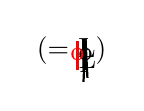
\begin{tikzpicture}[xscale=\myscalex-0.05,yscale=\myscaley-0.05]
\node (tone) at (3.5,0) {(= L)};
\node (syl) at (0,0) {\textsigma};
\node (syl2) at (2,0) {\red{\textsigma}};
\node (Rt) at (0,1) {o};
\node (H) at (-0.5,2) {L};
\node (R) at (0.5,3) {l};
\node (Rt2) at (2,1) {\red{o}};
\draw [thick] (syl.north) -- (Rt.south) ;
\draw [thick,red] (syl2.north) -- (Rt2.south) ;
\draw [thick] (Rt.north) -- (H.south) ;
\draw [thick] (Rt.north) -- (R.south) ;
\end{tikzpicture}
\end{minipage}
}

\newcommand{\OTLPolDef}{
\begin{minipage}{0.20\textwidth}
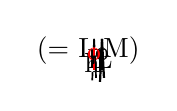
\begin{tikzpicture}[xscale=\myscalex-0.05,yscale=\myscaley-0.05]
\node (tone) at (3.5,0) {(= L.M)};
\node (syl) at (0,0) {\textsigma};
\node (syl2) at (2,0) {\red{\textsigma}};
\node (Rt) at (0,1) {o};
\node (H) at (-0.5,2) {L};
\node (R) at (0.5,3) {l};
\node (H2) at (1.5,2) {\epen{L}};
\node (R2) at (2.5,3) {\epen{h}};
\node (Rt2) at (2,1) {\red{o}};
\draw [thick] (syl.north) -- (Rt.south) ;
\draw [thick,red] (syl2.north) -- (Rt2.south) ;
\draw [thick] (Rt.north) -- (H.south) ;
\draw [thick] (Rt.north) -- (R.south) ;
\draw [semithick,dashed] (Rt2.north) -- (H2.south) ;
\draw [semithick,dashed] (Rt2.north) -- (R2.south) ;
\end{tikzpicture}
\end{minipage}
}

\newcommand{\OTLPolAlt}{
\begin{minipage}{0.20\textwidth}
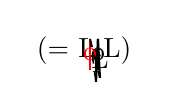
\begin{tikzpicture}[xscale=\myscalex-0.05,yscale=\myscaley-0.05]
\node (tone) at (3.5,0) {(= L.L)};
\node (syl) at (0,0) {\textsigma};
\node (syl2) at (2,0) {\red{\textsigma}};
\node (Rt) at (0,1) {o};
\node (H) at (-0.5,2) {L};
\node (R) at (0.5,3) {l};
\node (Rt2) at (2,1) {\red{o}};
\draw [thick] (syl.north) -- (Rt.south) ;
\draw [thick,red] (syl2.north) -- (Rt2.south) ;
\draw [thick] (Rt.north) -- (H.south) ;
\draw [thick] (Rt.north) -- (R.south) ;
\draw [semithick,dashed] (Rt2.north) -- (H.south) ;
\draw [semithick,dashed] (Rt2.north) -- (R.south) ;
\end{tikzpicture}
\end{minipage}
}

% Sec. 4.2, sixth tableau, polar questions with contour tones

\newcommand{\OTLLPolIn}{
\begin{minipage}{0.23\textwidth}
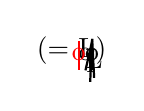
\begin{tikzpicture}[xscale=\myscalex-0.05,yscale=\myscaley-0.05]
\node (tone) at (5.2,0) {(= L)};
\node (syl) at (0,0) {\textsigma};
\node (syl3) at (3.4,0) {\red{\textsigma}};
\node (Rt) at (0,1) {o};
\node (Rt2) at (1.7,1) {o};
\node (Rt3) at (3.4,1) {\red{o}};
\node (H) at (-0.5,2) {L};
\node (R) at (0.5,3) {l};
\draw [thick] (syl.north) -- (Rt.south) ;
\draw [thick] (syl.north) -- (Rt2.south) ;
\draw [thick,red] (syl3.north) -- (Rt3.south) ;
\draw [thick] (Rt.north) -- (H.south) ;
\draw [thick] (Rt.north) -- (R.south) ;
\end{tikzpicture}
\end{minipage}
}

\newcommand{\OTLLPolDef}{
\begin{minipage}{0.23\textwidth}
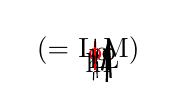
\begin{tikzpicture}[xscale=\myscalex-0.05,yscale=\myscaley-0.05]
\node (tone) at (5.2,0) {(= L.M)};
\node (syl) at (0,0) {\textsigma};
\node (syl3) at (3.4,0) {\red{\textsigma}};
\node (Rt) at (0,1) {o};
\node (Rt2) at (1.7,1) {o};
\node (Rt3) at (3.4,1) {\red{o}};
\node (H) at (-0.5,2) {L};
\node (R) at (0.5,3) {l};
\node (H3) at (2.9,2) {\epen{L}};
\node (R3) at (3.9,3) {\epen{h}};
\draw [thick] (syl.north) -- (Rt.south) ;
\draw [thick] (syl.north) -- (Rt2.south) ;
\draw [thick,red] (syl3.north) -- (Rt3.south) ;
\draw [thick] (Rt.north) -- (H.south) ;
\draw [thick] (Rt.north) -- (R.south) ;
\draw [dashed] (Rt3.north) -- (H3.south) ;
\draw [dashed] (Rt3.north) -- (R3.south) ;
\end{tikzpicture}
\end{minipage}
}

\newcommand{\OTLLPolSkip}{
\begin{minipage}{0.23\textwidth}
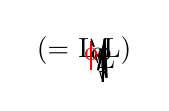
\begin{tikzpicture}[xscale=\myscalex-0.05,yscale=\myscaley-0.05]
\node (tone) at (5.2,0) {(= L.L)};
\node (syl) at (0,0) {\textsigma};
\node (syl3) at (3.4,0) {\red{\textsigma}};
\node (Rt) at (0,1) {o};
\node (Rt2) at (1.7,1) {o};
\node (Rt3) at (3.4,1) {\red{o}};
\node (H) at (-0.5,2) {L};
\node (R) at (0.5,3) {l};
\draw [thick] (syl.north) -- (Rt.south) ;
\draw [thick] (syl.north) -- (Rt2.south) ;
\draw [thick,red] (syl3.north) -- (Rt3.south) ;
\draw [thick] (Rt.north) -- (H.south) ;
\draw [thick] (Rt.north) -- (R.south) ;
\draw [dashed] (Rt3.north) -- (H.south) ;
\draw [dashed] (Rt3.north) -- (R.south) ;
\end{tikzpicture}
\end{minipage}
}  
  
\newcommand{\ilit}[1]{#1\il{#1}}    
\newcommand{\isit}[1]{#1\is{#1}}  

\makeatletter
\let\thetitle\@title
\let\theauthor\@author 
\makeatother

\newcommand{\togglepaper}[1][0]{ 
  \bibliography{../localbibliography}
  %% hyphenation points for line breaks
%% Normally, automatic hyphenation in LaTeX is very good
%% If a word is mis-hyphenated, add it to this file
%%
%% add information to TeX file before \begin{document} with:
%% %% hyphenation points for line breaks
%% Normally, automatic hyphenation in LaTeX is very good
%% If a word is mis-hyphenated, add it to this file
%%
%% add information to TeX file before \begin{document} with:
%% \include{localhyphenation}
\hyphenation{
affri-ca-te
affri-ca-tes
com-ple-ments
par-a-digm
Sha-ron
Kings-ton
phe-nom-e-non
Daul-ton
Abu-ba-ka-ri
Ngo-nya-ni
Clem-ents 
King-ston
Tru-cken-brodt
Tab-leau
cophono-logies
mark-edness
Ti-gri-nya
a-mong
Car-stens
Lu-bu-ku-su
}
\hyphenation{
affri-ca-te
affri-ca-tes
com-ple-ments
par-a-digm
Sha-ron
Kings-ton
phe-nom-e-non
Daul-ton
Abu-ba-ka-ri
Ngo-nya-ni
Clem-ents 
King-ston
Tru-cken-brodt
Tab-leau
cophono-logies
mark-edness
Ti-gri-nya
a-mong
Car-stens
Lu-bu-ku-su
}
  \papernote{\scriptsize\normalfont
    \theauthor.
    \thetitle. 
    To appear in: 
    Emily Clem,   Peter Jenks \& Hannah Sande.
    Theory and description in African Linguistics: Selected papers from the 47th Annual Conference on African Linguistics.
    Berlin: Language Science Press. [preliminary page numbering]
  }
  \pagenumbering{roman}
  \setcounter{chapter}{#1}
  \addtocounter{chapter}{-1}
}

\newcommand{\upstep}{\textupstep}


% \newcounter{tableauxcounter}

\renewcommand{\textltailn}{ɲ}
\renewcommand{\textbardotlessj}{ɟ}

\newcommand{\emphkh}[1]{\textit{#1}} %originally \textbf, banned by the guidelines



\definecolor{lsDOIGray}{cmyk}{0,0,0,0.45}


\newcommand{\xuparrow}[1]{%
  {\left\uparrow\vbox to #1{}\right.\kern-\nulldelimiterspace}
}
\renewcommand \textupstep[1]{\char"A71B#1}
\renewcommand \textdownstep[1]{\char"A71C#1}
 
 \newcommand{\ꜛ}{\textsf{ꜛ}}
 
\def\biberror{\undefined}


\newcommand{\OTbox}[1]{\resizebox{.88\textwidth}{!}{#1}}
 
\usepackage{pifont.sty}

\author{Wm. G. Bennett\affiliation{University of Calgary and Rhodes University}}
\title{‘Backwards’ sibilant palatalization in a variety of Setswana}
\abstract{Palatalization of coronals and stridents is well-known and widespread, and is most commonly associated with front vowels or glides as triggers. In some dialect(s) of Setswana, a much different type of palatalization occurs: alveolar stridents /s ts tsʰ/ become pre-palatal [ʃ tʃ tʃʰ] before back vowels and the glide [w]. Clear empirical support for this pattern comes from productive alternations induced by the nominalizing suffix /-ɔ/, as well as alternations with an assortment of less productive morphemes, and lexical evidence. If palatalization before front vocoids is phonetically natural, then palatalization before back vocoids seems like it must be phonetically unnatural. However, this paper suggests that it is not the case: palatalization before back vowels actually makes phonetic sense, as a consequence of using lip rounding as a phonetic enhancement of the S~Š distinction.}
%\end{styleHeading}
\begin{document}
\maketitle
\section{Introduction}\label{sec:bennett:1}
\subsection{The puzzle}\label{sec:bennett:1.1}

% \abstract{Palatalization of coronals and stridents is well-known and widespread, and is most commonly associated with front vowels or glides as triggers. In some dialect(s) of \ili{Setswana}, a much different type of palatalization occurs: alveolar stridents /s ts tsʰ/ become pre-palatal [ʃ tʃ tʃʰ] before back vowels and the glide [w]. Clear empirical support for this pattern comes from productive alternations induced by the nominalizing suffix /-ɔ/, as well as alternations with an assortment of less productive morphemes, and lexical evidence. If palatalization before front vocoids is phonetically natural, then palatalization before back vocoids seems like it must be phonetically unnatural. However, this paper proposes that it is not the case: palatalization before back vowels actually makes phonetic sense, as a consequence of using lip rounding as a phonetic enhancement of the S~Š distinction.}


Palatalization of coronals and of stridents is well-known and widespread, and is most commonly associated with high front vowels/glides as triggers (\citealt{Bateman:2007aa,Bateman2010,Kochetov2011}; etc.). A common example is \ili{Japanese}, in which the native lexical stratum exhibits allophony of [s] and [ʃ] depending on the following vowel: [s] occurs generally, but appears as [ʃ] before [i]. Similar patterns are reported in a vast number of languages; \citet{Bateman:2007aa} lists at least \ili{Nupe}, \ili{Korean}, \ili{English}, \ili{Mandarin} \ili{Chinese}, \ili{Hausa}, Mina, Romanian, Moldavian, and \ili{Yagua} as having similar alternations. \citep[from][]{Cole1955}

This sort of [s]→[ʃ]/ {\longrule} i alternation makes a lot of sense. It makes sense articulatorily in that [i] requires the tongue body to be elevated and close to the palate, while [s] requires the tongue body to be much lower, such that the tip forms a constriction. Thus, it seems reasonable that [s] should be harder to produce than [ʃ] before [i], so we might expect to find the former turning into the latter in that context. This alternation also makes acoustic sense: in the sequence [si], coarticulation between the [s] and [i] should make [s] sound more like [ʃ]. This is because retraction of the tongue blade (to position the blade to produce [i]) increases the length of the cavity in front of the frication. This should shift the noise spectrum of [s] downward, towards that of [ʃ]. So, a s→ʃ alternation before a high front vocoid is phonetically natural, which seems to fit nicely with how common such processes are cross-linguistically.

Some varieties of \ili{Setswana} give us a glimpse of a very different sort of pattern. In general, [s] and [ʃ] contrast \REF{ex:bennett:1}. The examples in \REF{ex:bennett:2} show underlying /s/ changing into [ʃ] before [ɔ].\footnote{While Cole describes this merely as ‘\ili{Setswana}’, it seems to obtain only for certain Southern dialects, and not for standard \ili{Setswana}. See \sectref{sec:bennett:2.1} and \sectref{sec:bennett:2.6} for more discussion.}

\ea\label{ex:bennett:1}
s and ʃ are contrastive in \ili{Tswana} \citep[25]{Cole1955}\\
\downingdouble{-sɛba}{-ʃɛba}
\downingdouble{‘slander’}{‘look round’}
\z

\ea\label{ex:bennett:2}
\langinfo{}{}{s → ʃ / {\longrule} ɔ (!)}
\ea\label{ex:bennett:2a}
\downingdouble{-hisa}{sɪ-hiʃɔ}
\downingdouble{‘burn’}{‘burner’}
\ex\label{ex:bennett:2b} 
\downingdouble{-ɔmisa}{sɪ-wɔmiʃɔ}
\downingdouble{‘dry’}{‘dryer’}
\ex\label{ex:bennett:2c} 
\downingdouble{-busa}{m-muʃɔ}
\downingdouble{‘govern’}{‘government’}
\z
\z

If the s→ʃ/ {\longrule} i pattern makes sense, then these examples seem downright weird. Here, we observe the same s→ʃ alternation induced by a vowel that is low and back, not high and front. This pattern is not merely s→ʃ, but rather \textit{S→Š}: it holds for all the strident affricates and fricatives alike (as §2 will demonstrate).

The weirdness of this data makes it interesting. A large body of current work appeals to phonetic naturalness as a guiding factor in phonological systems, in various forms. For instance, \citet{Hayes1999} argues that phonological constraints are functionally motivated, and must be phonetically sensible. \posscitet{Steriade2008} P-map proposal, similarly, posits that input-output changes are moderated by perceptual distance, such that phonetically sensible changes are preferred. And the entire body of literature under the banner of ‘evolutionary phonology’
%\textstyleFootnoteSymbol{}
\footnote{(\citealt{Ohala1981,Ohala1990,Ohala:2004aa}, etc.; rehashed and renamed by \citealt{Blevins2004})} takes phonological patterns to be the direct result of phonetically-driven changes, coupled with morpho-phonological analogy. The pattern we observe in \REF{ex:bennett:2} seems phonetically as \textit{un-natural} as can be, in that it is virtually the opposite of a pattern that is phonetically well-motivated. Instead of a high front vowel [i], we observe a relatively low back vowel [ɔ] causing palatalization.\footnote{A more direct opposite of [i] would be the vowel [ɑ], but this does not exist in \ili{Setswana}.} As §2 will show, this is not a behaviour unique to [ɔ]; other back vowels also induce the same S→Š/ {\longrule} U alternations.

Palatalization before back vocoids is not unprecedented. For instance, \citet[68]{Bateman:2007aa} notes palatalization before [u] in Tohono O’Odham. But, cross-linguistic surveys of palatalization (\citealt{Bateman:2007aa,Kochetov2011}) consistently find that high front vocoids are the ‘best’ triggers for palatalization. If palatalization is triggered by a back vocoid like [u], then front vocoids also trigger palatalization. Indeed, the generalization that Bateman reports for Tohono O’Odham is that palatalization is triggered not only by [u], but also by [i] and [e]. This dovetails with an observation (made by Bateman and Kochetov alike) that higher vocoids are better palatalization triggers. In other words, cases like Tohono O’Odham show palatalization only before \textit{high} back vocoids (which [ɔ] definitively isn’t), and high front vocoids also trigger the same palatalization.
% Edwin: Missing reference for Bennett & Braver 2015 and Kotzé & Zerbian 2007
A further pertinent fact is that many Southern \ili{Bantu} languages have palatalization triggered by [w] (\citealt{Louw1975,Ohala1978,Herbert1990,Bennett2015,Bennett&Braver2016}, etc.).  However, this phenomenon preferentially targets bilabials for palatalization, and only marginally applies to non-labials; it therefore seems dissimilatory in nature. Some previous analyses argue that it isn’t dissimilation (e.g. \citealt{Kotze&Zerbian2008}, by instead positing that the palatalization is really triggered by an /i/ or /j/ (which is typically covert). Neither of these lines of reasoning lead to a plausible analysis of the \ili{Setswana} examples in \REF{ex:bennett:2}. The /sɔ/→[ʃɔ] alternation is not obviously dissimilatory. There is also no evidence for a covert front vocoid in these examples, and indeed front vocoids in \ili{Setswana} do not otherwise cause palatalization of /s/ (cf. (\ref{ex:bennett:2}a): sɪ-hiʃɔ, *ʃɪ-hiʃɔ).

The question at hand, then, is how to understand the S→Š/ {\longrule} U pattern seen in \REF{ex:bennett:2}. Is this data reflective of a real process? If so, is it phonetic, phonological, or morphological? If it seems so squarely the opposite of a well-understood and phonetically natural pattern (S→Š/ {\longrule} i), why and how does it also exist?

\subsection{The proposal}\label{sec:bennett:1.2}

The main claims of this paper are three. The first is that S→Š palatalization before back vowels is robust and productive in at least some variety of \ili{Setswana}. The second is that the alternation seems entirely sensible when viewed from another angle: lip rounding may be a reason to prefer Š over S before back vocoids. This leads to the third claim: if phonetics informs phonology, it does so in a non-deterministic way. S→Š/ {\longrule} U is the opposite of well-understood S→Š/ {\longrule} I alternations, in that it is triggered by back vowels instead of front vowels. Moreover, it seems intuitively unlikely that any language could have both S→Š/ {\longrule} I and S→Š/ {\longrule} U, because the occurrence of the one undermines the evidence for the other. 

If opposite phonological patterns can \textit{both} be phonetically natural, then phonetic naturalness cannot in principle give us a complete understanding of phonology.

The paper is structured as follows. \sectref{sec:bennett:2} presents the \ili{Setswana} S→Š process in further detail. \sectref{sec:bennett:3} observes that the phenomenon does not appear to be unique to this language: parallels can be found in a few other \ili{Bantu} languages, and perhaps further afield. \sectref{sec:bennett:4} presents rounding as a potential basis for S→Š being phonetically natural before back vocoids like [ɔ]. \sectref{sec:bennett:5} concludes and observes some of the broader ramifications.

\section{Data and Support}\label{sec:bennett:2}

\subsection{Background about the data}\label{sec:bennett:2.1}

\ili{Setswana} (a.k.a. \ili{Tswana}) is a southern \ili{Bantu} language (Guthrie S.50) spoken mainly in northern South Africa and Botswana. Examples marked as ‘own data’ were collected by the author, with the help of a native-speaker consultant from Taung, North-West Province, South Africa. This speaker did not report a specific name for his idiolect, but did report being clearly aware that his accent is typical of that area, and is non-standard.\footnote{I thank Thabo Ditsele, Andy Chebanne, and an anonymous reviewer for confirming that \ili{Setswana} dialects from further east (Gauteng) and north (Botswana) do not exhibit this S→Š pattern.} Additional data comes from other sources on \ili{Setswana}, chiefly \posscitet{Cole1955} grammar (no specific dialect information is at hand for most of Cole’s data). For lack of a better name, I will refer to the dialect(s) represented in these sources of data simply as ‘\ili{Setswana}’; but it should be noted that standard, prescriptive, \ili{Setswana} does not exhibit the patterns described here.\footnote{For instance, the University of \posscitet{University-of-Botswana:2001aa} \textit{Sound System of Setswana} does not mention the S→Š alternation as part of the phonology.} On the basis of a dialect comparison by \citet{Malepe1966}, it seems that this is a characteristic found only in southern dialects, including those that Malepe calls \ili{Rolong}, \ili{Tlhaping}, and \ili{Tlharo}, though further research is needed to verify how geographically widespread the phenomenon is.

The consonant inventory of \ili{Setswana} is given in \tabref{tab:bennett:1} %
%The style guide says no vertical lines, but I think for a consonant inventory it makes more sense to keep them.
 (\citealt{Bennett2016}; see also \citealt{Cole1955}; \citealt{chebanneetal1997}, U. \citealt{University-of-Botswana:2001aa}). Consonants in parentheses are marginal. Unaspirated stops and affricates may be realized as ejectives (apparently in \isi{free variation}). The affricate [qχ] is often analyzed as /qʰ/ or /kxʰ/, and [χ] is often characterized as /x/ (\citealt{Cole1955}, etc.; see \citealt{Bennett2016} for further discussion and data).
 
\begin{table}
\begin{tabularx}{\textwidth}{XXXXcXXXX}
\lsptoprule

p pʰ   b &  & t   tʰ   d &  &  &  & k  kʰ &  & (ʔ)\\
&  & ts tsʰ & tɬ   tɬʰ & tʃ   tʃʰ  dʒ &  &  & qχ & \\
& (f) & s &  & ʃ &  &  & χ & h \\
m &  & n &  &  & ɲ & ŋ &  & \\
&  & r &  &  &  &  &  & \\
w &  &  & l &  & j &  &  & \\
\lspbottomrule
\end{tabularx}
\caption{Consonant inventory of Setswana}
\label{tab:bennett:1}
\end{table}

The \isi{vowel inventory} is given in \figref{fig:bennett:1} \citep{Bennett2016}. The vowel system has at least four contrastive degrees of height, possibly more.\footnote{This is a slight simplification. The transcriptions given here follow \posscitet{Cole1955} orthographic ones, which do not generally reflect a \isi{vowel harmony} process that produces raised counterparts of each pair of mid vowels; see \citet{Dichabe1997} for further details on this harmony. Some sources claim that some or all of these additional degrees of height are not merely derived, but are also contrastive in that they occur in contexts not explainable by the \isi{vowel harmony} (for example, see \citealt{chebanneetal1997,Creissels2005emergence}, and also \citealt{Khabanyane1991} on Southern \ili{Sotho}).} To avoid a deluge of diacritics, the semi-close vowels [e̝ o̝] are rendered as ‘ɪ’ and ‘ʊ’ in all examples (rather than ‘e’ and ‘o’ as in the standard orthography and some previous transcriptions like those of \citealt{Cole1955}; see also \citealt{Roux2008} for finer acoustic details). The tonal system of \ili{Setswana} is complex and involves numerous alternations (see \citealt{chebanneetal1997} for an overview); as such, tones are not marked in the single-word examples given here. As far as I can tell, they do not affect the consonantal alternations of interest here.

   
\begin{figure}
% \includegraphics{figures/bennettFig1.png}
\begin{vowel}
 \putcvowel{i}{1}
 \putcvowel{e̝}{2}
 \putcvowel{ε}{3}
 \putcvowel{a}{4}
 \putcvowel{ɔ}{6}
 \putcvowel{o̝}{7}
 \putcvowel{u}{8}
\end{vowel}
\todo[inline]{Note that [a] is front in this chart, while it is central in the original. IPA has no symbol for an open central unrounded vowel. There are three possibilities: 1) use [a] in its canonical position, i.e. in front 2) use a diacritic like centralized [ä] or retracted [a̠] in the central position 3) use [a] in central position, leading to a mismatch between IPA conventions and the conventions used in this paper}
\caption{Vowel inventory of Setswana \citep{BennettEtAl2016}}
\label{fig:bennett:1}
\end{figure} 

\subsection{On S and Š}\label{sec:bennett:2.2}

The \isi{focus} of interest for this paper is palatalization of stridents before back vocoids, characterized in shorthand as S→Š/ {\longrule} U. The ‘S’ denotes all anterior stridents, whether they appear alone or in NC sequences: \{s ts tsʰ ns nts ntsʰ\}. The ‘Š’ likewise denotes posterior stridents: \{ʃ tʃ tʃʰ nʃ ntʃ ntʃʰ\}. The ‘U’ denotes back vowels and glides: \{ɔ ʊ u w\}. There is no evidence that the voiced posterior affricate [dʒ] participates in the pattern; this is consistent with the absence of [z ʒ] from the native consonant inventory.

\subsection{Productive, synchronic S{\textasciitilde}Š alternations}\label{sec:bennett:2.3}

The examples from \sectref{sec:bennett:1} point to a neutralizing pattern. That is, S and Š are normally contrastive, and we find S→Š, but not the reverse Š→S. The most robust and productive source of synchronic S{\textasciitilde}Š alternations comes from nominalizations formed with the suffix /-ɔ/. Some examples are given below in \tabref{tab:bennett:2}. For /tsʰ/ → [tʃʰ], it’s difficult to find examples showing this alternation because /tsʰ/ is relatively uncommon in stem-final position. But, it can be derived in irregular causatives; these forms do show S→Š/ {\longrule} U in the expected fashion.

\begin{table}
\small
\begin{tabularx}{\textwidth}{l@{~}l@{~}Q@{}l@{~}Q}
\lsptoprule
\multicolumn{5}{c}{/s/→[ʃ]}\\
\midrule
-hisa & ‘burn’ & sɪ-hiʃɔ & ‘burner’ & (own data)\\
-ɔmisa & ‘dry sth.’ & sɪ-wɔmiʃɔ & ‘dryer’ & (own data)\\
-busa & ‘govern’ & m-muʃɔ & ‘government’ & \citep[77]{Cole1955}\\
-tʰusa & ‘assist’ & tʰuʃɔ & ‘assistance’ & \citep[90]{Cole1955}\\
\midrule
\multicolumn{5}{c}{/ts/→[tʃ]}\\
\midrule
-bitsa & ‘call’ & pitʃɔ & ‘a call’ & (own data)\\
-χɔpʊtsa & ‘remind’ & sɪ-χɔpʊtʃɔ & ‘reminder’ & \citep[86]{Cole1955}\\
-lɔɔtsa & ‘whet, sharpen’ & tɔɔtʃɔ & ‘whetstone’ & \citep[90]{Cole1955}\\
-bʊtsa & ‘ask’ & pʊtʃɔ & ‘question’ & \citep[90]{Cole1955}\\
-itsɪ & ‘know’ & kitʃɔ & ‘knowledge’ & \citep[90]{Cole1955}\\
-ikʊkʊbɛtsa & ‘stoop (refl, caus)’ & bʊ-ikʊkʊbɛtʃɔ & ‘humility’ & \citep[205]{Cole1955}\\
-iɲatsa & ‘despise (refl)’ & iɲatʃɔ & ‘self-disparagement’ & \citep{Cole1955}\\
\midrule
\multicolumn{5}{c}{/tsʰ/→[tʃʰ]}\\
\midrule
-bɔntsʰa & ‘show’ & pɔntʃʰɔ & ‘a showing’ & (own data; cf. bona ‘see’)\\
-tɬʰalɪfa & ‘become wise’ & -tɬʰalɪtsʰa,\newline -tɬʰalɪtʃʰwa & ‘make wise’ & \citep[205]{Cole1955}\\
\lspbottomrule
\end{tabularx}
\caption{Productive S→Š alternations in /-ɔ/ nominalizations}
\label{tab:bennett:2}
\end{table}

The S{\textasciitilde}Š alternations we see here are not characteristic of nominalizations in general. Agentive nominalizations are formed with a suffix /-i/, and these don’t exhibit the same alternation (cf. -tʰusa ‘help’ > mʊ-tʰusi ‘assistant, helper’; *mʊ-tʰuʃi). As such, the S{\textasciitilde}Š alternation evident in these forms must be due to the presence of the vowel [ɔ]. This is corroborated by other morphemes that also show the same related S{\textasciitilde}Š pattern.

\subsection{S→Š in other morphological contexts}\label{sec:bennett:2.4}

The S{\textasciitilde}Š alternation can also be observed in certain pronominal concords; examples are given in \tabref{tab:bennett:3} below (from \citealt{Cole1955}). The first set of forms are pronouns, demonstratives, and quantifiers with class 8/10\footnote{Classes 8 and 10 are homophonous, so I will not distinguish them here.} concord. In pronominal stems that have front vocoids like [ɛ], class 8/10 forms always have [ts]. However, class 8/10 forms have [tʃ] when the following vowel is [ɔ], manifesting the S→Š/ {\longrule} U pattern. The second set of forms show class 7 behaving the same way: we find [s] in class 7 forms generally, but [ʃ] before [ɔ]. (These pronominal stems are few in number, and phonotactically non-diverse; in reading \posscitet{Cole1955} grammar, I was unable to find any that have other vocoids.

\begin{table}
\begin{tabularx}{\textwidth}{llQll}
\lsptoprule
Class 8/10: & ts before ɛ &  & tʃ before ɔ & \\
\midrule
& tsɛ & ‘this’ & tʃɔnɛ & ‘they’\\
& tsɛʊ & ‘that’ & tʃɔsi & ‘only they’\\
& tsɛnʊ & ‘that one’ & tʃɔɔpɛdi & ‘both’\\
& tsɛlɛ & ‘that one yonder’ & tʃɔtɬʰɛ & ‘all’\\
& muxatsɛ & ‘his/her spouse’ & muxatʃɔ & ‘your spouse’\\
% % &  &  &  & \\
\midrule
Class 7: & s before ɛ &  & ʃ before ɔ & \\
\midrule
& sɛ & ‘this’ & ʃɔnɛ & ‘it’\\
& sɛʊ & ‘that’ & ʃɔsi & ‘only it’\\
& sɛnʊ & ‘that one’ & tʃɔtɬʰɛ & ‘all’\\
& sɛlɛ & ‘that one yonder’ &  & \\
\lspbottomrule
\end{tabularx}
\caption{S{\textasciitilde}Š alternations in pronominal stems\label{tab:bennett:3}}
\end{table}

We can also observe S→Š/ {\longrule} U in certain verbal suffixes. One is the reversive verb extension, variously /-ʊl-/ or /-ʊlʊl-/ \REF{ex:bennett:3} (\citealt{Cole1955}:212ff). The form in (\ref{ex:bennett:3}a) looks on the surface like an applicative structure /-tsʰ-ɛl-a/, based on a root /-tsʰ-/ (which is not attested by itself). Related stems that have the reversive extension instead of the applicative one have [tʃʰ] instead of [tsʰ] (3b,c).

\ea\label{ex:bennett:3}
\langinfo{}{}{Reversive verb extension}
\ea\label{ex:bennett:3a}

\downingdouble{-tsʰɛla}{‘pour’}
\ex\label{ex:bennett:3b}

\downingdouble{-tʃʰʊla}{‘serve, dish out food’}
\ex\label{ex:bennett:3c}

\downingdouble{-tʃʰʊlʊla}{‘spill’}
\z
\z

The passive suffix also shows evidence for the same S→Š/ {\longrule} U alternation, albeit in a less simple way. This is illustrated in \REF{ex:bennett:4} and \REF{ex:bennett:5}, based on data and observations from \citet[193--195]{Cole1955}. The basic form of the passive is /-w-/ (\ref{ex:bennett:4}a). However, Cole reports that the same extension is normally realized instead as /-iw-/ after roots ending with \{s ts tsʰ\} (\ref{ex:bennett:4}b); roots ending with /ts/ additionally change the /ts/ into [d] (\ref{ex:bennett:4}c). This is not direct evidence for the S→Š/ {\longrule} U alternation, but the allomorphy is clearly phonotactically-based, and systematically fails to produce surface SU sequences.

\ea\label{ex:bennett:4}
\langinfo{}{}{Passive suffix allomorphy (\citealt{Cole1955}:193ff)}
\ea\label{ex:bennett:4a}

-bɔn-a  >  -bɔn-w-a

     ‘see’
\ex\label{ex:bennett:4b}

-bɛs-a  >  -bɛs-iw-a

     ‘roast’
\ex\label{ex:bennett:4c}

-bits-a  >  -bid-iw-a

     ‘call’\\
\z
\z

Furthermore, \citet{Cole1955} does note that some Eastern dialects of \ili{Setswana} use /-w-/ instead of /-iw-/ in these instances. In those forms, we \textit{do} find the S→Š/ {\longrule} U alternation, occurring just as expected \REF{ex:bennett:5}. Thus, the passive suffix allomorphy avoids creating SU sequences; where it does create them, we find S→Š as usual.

\ea\label{ex:bennett:5}
\langinfo{}{}{\ili{Setswana}: Eastern dialects \citep{Cole1955}}\\
\ea\label{ex:bennett:5a}

-bɛs-iw-a {\textasciitilde} -bɛʃ-w-a

     ‘be roasted’\\
\ex\label{ex:bennett:5b}

-bid-iw-a  {\textasciitilde} -bitʃ-w-a

     ‘be called’\\
\z
\z
Palatalization can also be observed with the diminutive suffix /-ana/, which\linebreak causes a host of changes to preceding consonants (for further details and discussion, see \citealt{Cole1955,Louw1975,Herbert1990,Bateman:2007aa,Kotze&Zerbian2008}). The generalization of note here is that some of these changes can derive stridents from other, non-strident, consonants. These derived consonants follow the same S→Š alternation we see elsewhere. This is illustrated in \REF{ex:bennett:6}: /d/ changes to [ts] generally (\ref{ex:bennett:6}a), but to [tʃ] when it precedes a back vocoid (\ref{ex:bennett:6}b). 

\ea\label{ex:bennett:6}
\langinfo{}{}{S→Š in diminutives \citep{Cole1955}}\\
\ea\label{ex:bennett:6a}

pʊdi  → puts-ana

     ‘goat’\\
\ex\label{ex:bennett:6b}

lɪ-χɔdu  → lɪχɔtʃw-ana

     ‘thief’\\
\z
\z

\subsection{Further lexical evidence}\label{sec:bennett:2.5}


We can also observe the S→Š/ {\longrule} U pattern in the lexicon. One source of evidence is from lexical doublets. These substantiate the same observation made about the diminutives above: when something changes a consonant into S, it also changes into Š before U. \citet[83ff]{Cole1955} notes that certain nouns of class 5/6 have doublets, one with [ts] or [s], the other with \{b l d r h χ\}. \tabref{tab:bennett:4} gives some examples of this variant S (mainly drawn from \citealt{Cole1955}:83ff); for example, the first one [lɪ-tsats] ‘sun, day’ has [ts], while the usual \isi{plural form} Cole reports is [ma-latsi], with [l] instead.

\begin{table}
\begin{tabularx}{\textwidth}{llXX}
\lsptoprule

-latsi & lɪ-tsatsi (cf. pl. ma-latsi) & ‘sun, day’ & (l {\textasciitilde} ts)\\
-dibʊχɔ & lɪ-tsibʊχɔ & ‘ford’ & (d {\textasciitilde} ts)\\
-bɛlɛ & lɪ-tsɛlɛ & ‘breast’ & (b {\textasciitilde} ts)\\
-rapɔ & lɪ-sapɔ & ‘bone’ & (r {\textasciitilde} s) \\
-rama & lɪ-sama & ‘cheek’ & \\
\lspbottomrule
\end{tabularx}
\caption{Lexical doublets with S}
\label{tab:bennett:4}
\end{table}

When a back vowel follows the initial consonant of the root, we do not find doublets with S; instead, they have Š. This is illustrated in table 5 (examples again from \citealt{Cole1955}).\footnote{\citet[83]{Cole1955} notes some exceptional forms that deviate from this generalization in minor ways. For example, [lɪ-saχɔ] ‘buttock’ is listed with variant forms [lɪ-tsʰaχɔ {\textasciitilde} lɪ-ʃaχɔ]. No [ʃ] is expected here, since the following vowel is [a]. But, interestingly, the plural is only given with [s], as [ma-saχɔ].}
%TODO Remind Peter that ɔ has a problem of typesetting, I don't see it.
\begin{table}
\begin{tabularx}{\textwidth}{lllX}
\lsptoprule

-bɔχɔ & lɪ-tʃɔχɔ
(cf. pl. ma-bɔχɔ) & ‘arm’ & (b {\textasciitilde} tʃ before U)\\
-bʊlɪ & lɪ-tʃwɪlɪ & ‘fist’ & \\
-rɔpʰi & lɪ-ʃɔpʰi & ‘blister’ & (r {\textasciitilde} ʃ before U)\\
-rʊpe & lɪ-ʃʊpe & ‘ruin’ & \\
-rʊʊ & lɪ-tʃʰʊʊ & ‘paw’ & \\
-χɔdi & lɪ-ʃɔdi & ‘starling’ & (χ {\textasciitilde} ʃ before U)\\
-hulɔ & lɪ-ʃulɔ & ‘foam, froth’ & (h {\textasciitilde} ʃ before U)\\
-hudu & lɪ-ʃudu & ‘hole for stamping corn’ & \\
\lspbottomrule
\end{tabularx}
\caption{Lexical doublets have Š instead of S before U}
\label{tab:bennett:5}
\end{table}

Additional support for S→Š/ {\longrule} U comes from the distribution of stridents in the lexicon. The occurrence of SU, i.e. \{s ts tsʰ\} before a back vocoid, seems to be vanishingly rare. Some examples of SU forms are attested in Cole’s grammar, but many are presented as variant forms that may also be realized with Š. A few words systematically must have SU (not ŠU), but are clearly loanwords. These are illustrated in \tabref{tab:bennett:6} below. It is worth noting, however, that there are also loanwords where source S \textit{does} neutralize to Š before U. Such forms cannot be attributed by some general characteristic of the treatment of loanwords, because loans with [s] before non-back vocoids normally retain it faithfully as [s] (as in ‘stool’ in \tabref{tab:bennett:6}).

\begin{table}
\begin{tabularx}{\textwidth}{XXX}
\lsptoprule
\multicolumn{3}{c}{Exceptional SU sequences in loanwords}\\
\midrule 
lɪ-tsula  & ‘\ili{Zulu} person’ & < \ili{Zulu}\\
{\textasciitilde} lɪ-sʊlʊ \\
{\textasciitilde} lɪ-zʊlʊ \\
pɔsɔ & ‘post office’ & < \ili{Afrikaans}\\
dʒɛsu & ‘Jesus’ & \\
zuu & ‘zoo’ & \\
\midrule
\multicolumn{3}{c}{Loanwords with non-exceptional S→Š/ {\longrule} U}\\
\midrule
lɪ-ʃɔlɛ & ‘soldier’ & s→ʃ neutralization\\
ʃukiri & ‘sugar’ & \\
sɪ-tulɔ & ‘stool’ & normally s→s\\
\lspbottomrule
\end{tabularx}
\caption{Sporadic S→Š/ {\longrule} U in loanwords}
\label{tab:bennett:6}
\end{table}

In the native lexicon, Š may occur before any of the vowels: \{ʃ tʃ tʃʰ\}are not as restricted as \{s ts tsʰ\}. Some examples of Š before non-back vowels are given in \tabref{tab:bennett:7} below (from \citealt{Cole1955}). 

% TODO Ask how to fix ugliness of tabularx?!?!?!?!?
\begin{table}[p]
\begin{tabularx}{\textwidth}{XXX}
\lsptoprule 
{Ši} & ma-ʃi & {‘milk’} \\ 
\tablevspace
{Šɪ} & di-ʃaʃɪ & {‘coward’} \\
& mʊ-ʃɪ & ‘meerkat’ \\
& -ʃɪna & ‘(to) bare teeth’  \\
& ntʃʰɪ & ‘ostrich’  \\
& bʊ-ratʃʰɪ & ‘brush’ \\ 
\tablevspace
 {Šɛ} & -ʃɛba & {‘(to) look round’} \\
& ʃɛlɛŋ & ‘shilling’ \\ 
\tablevspace
{Ša} &-ʃa & {‘disperse’ (of mist)} \\
& -ʃa & ‘(to) burn (unacc.)’  \\
&-ʃa(j)a & ‘give child a name’ \\ 
&-ʃa & ‘new’ \\ 
&mʊ-ʃa & ‘young person’ \\ 
&-ʃaqχala & ‘become angry’ \\ 
&ntʃa & ‘dog’ \\ 
&-tʃʰa & ‘dry up (unacc.)’ \\ 
&sɪ-tʃʰaba & ‘nation, tribe’ \\
\lspbottomrule
\end{tabularx}
\caption{Š may occur before non-back vowels \citep{Cole1955}}
% \todo[inline]{check table with author}
\label{tab:bennett:7}
\end{table}

\begin{table}[p]
\begin{tabularx}{\textwidth}{XXXX}
\lsptoprule
& Front \{i ɪ ɛ\} & Central \{a\} & Back \{u ʊ ɔ\}\\
\midrule
S \{s ts tsʰ\} & common & uncommon & very rare\\
Š \{ʃ tʃ tʃʰ\} & uncommon & common & common\\
\lspbottomrule
\end{tabularx}
\caption{Impressionistic trends in the distribution of S and Š before front, central, and back vowels}
\label{tab:bennett:8}
\end{table}

The preponderance of examples in \tabref{tab:bennett:7} show Š before [a], rather than the other non-back (i.e. front) vowels. This is not an accident of presentation, but reflects the trend in the data that \citet{Cole1955} provides. Š seems more common before [a] than before front vowels. ŠI sequences (where ‘I’ stands for front vowels) also seem less common than SI sequences, but they are not nearly as rare as ŠU. These observations, consolidated in table 8, are based on my own impressions of data collected first-hand, as well as examination of \posscitet{Cole1955} data. \pgposscitet{Cole1955}{35} description of the relationship between S and Š agrees with my impressions.



The generalization that SU sequences are almost completely absent from the lexicon suggests that the S→Š/ {\longrule} U generalization is not merely part of the morpho-phonology of the language, but also holds over the lexicon as a phonotactic generalization. The observation that Š is more common before back vowels than front vowels is not obviously expected. It is conceivable that Š is over-represented before back vowels because the S→Š/ {\longrule} U neutralization derives Š in this context, but more extensive quantitative study is needed to be sure.

\subsection{Historical and comparative support}\label{sec:bennett:2.6}

Finally, there is also historical and comparative evidence that corroborates the S→Š/ {\longrule} U pattern. According to \pgposscitet{Malepe1966}{67ff} dialect survey and comparative analysis, the \ili{Rolong}, \ili{Tlhaping}, and \ili{Tlharo} dialects underwent a historical change *S > Š/ {\longrule} \{u ʊ ɔ\}. Evidence for this change comes from dialect variation of exactly the sort expected based on the lexical variation seen so far. For example, Malepe identifies ‘hearth’ as [lɪ-iʃɔ] in the \ili{Rolong} dialect, but [lɪ-isɔ] in \ili{Kwena} and other dialects. There is no S{\textasciitilde}Š dialect variation before front vowels.\footnote{\citet{Malepe1966} characterizes \ili{Rolong}, \ili{Tlharo} and \ili{Tlhaping} as Southern dialects. He identifies the hometown of the primary consultant, Taung, as a \ili{Tlhaping} area. Another consultant I worked with came from Kuruman, which Malepe notes as a \ili{Tlharo} area.}

The point: circumstantial evidence confirms that the S{\textasciitilde}Š alternations seen above are a change \textit{from} S, \textit{to} Š – a change conditioned by \textit{back} vocoids. It is not the case that there is back-and-forth allophony with no contrast. Nor is it the case that the alternating stridents were historically *Š, with de-palatalization or fronting induced by front vowels. 

\section{Parallels elsewhere?}\label{sec:bennett:3}

\ili{Setswana} is not alone in having a ‘backwards’ distribution of Š and S before vowels. A similar pattern is reported much further north, for \ili{Haya} and \ili{Nkore-Kiga}, two \ili{Bantu} languages spoken in Tanzania and Uganda. In both languages, the reported pattern is that [s z] occur before /i/, while [ʃ ʒ] occur before /e a o u/ (\citealt{Byarushengo1975,Hyman2003b}; see also \citealt{Hansson2001,Hansson2010}). This is more narrowly the opposite of patterns like the \ili{Japanese} one, with a split between the high front vowel [i] versus all the other vowels.

In the \ili{Haya} and \ili{Nkore-Kiga} cases the origin of the ‘backwards’ pattern seems to be morphological. \posscitet{Hyman2003b} analysis of the S{\textasciitilde}Š alternations in \ili{Haya} is that Proto-\ili{Bantu} *c spirantized to [s] before the short causative *-i̝-, and the causative *-i̝- was absorbed in the process, yielding a string of changes *c-i̝- > sj > [s].\footnote{See also \citet{Bennett&Pulleyblank:2014} for an argument that morphology is a major factor in the synchronic distribution of [s] and [ʃ] in \ili{Nkore-Kiga}.} This resulted in synchronic s{\textasciitilde}ʃ alternations between related verb stems, e.g. [-ʃáaʃ-a] ‘hurt (intransitive)’ vs. [-ʃáas-a] ‘hurt (transitive)’ \citep[85]{Hyman2003b}. The stem-final [s] in the latter form is due to the historical presence of *-i̝-, while the unaffixed form retains [ʃ]. Such alternations were then generalized by analogy, in effect treating all s-final stems as ‘pseudo-causatives’.

The \ili{Setswana} pattern is clearly not morphological in this way, however: it seems entirely phonotactic in nature. The S{\textasciitilde}Š alternation can be seen in a wide range of morphemes, and even root-internally. This includes many situations where any kind of spirantizing influence of a historical superhigh vowel is implausible, e.g. in demonstratives, possessives, and /-ɔ/ nominalizations. In short, the \ili{Setswana} pattern is clearly not due to front vocoids; not historically, and not synchronically.

Examples of other languages more in line with \ili{Setswana}, with \textit{phonotactic} s{\textasciitilde}ʃ patterns induced by back vocoids, are less abundant. However, there is a possible example in \ili{Tigrinya}\footnote{I thank Sharon Rose for pointing this example out to me.}: numerals exhibit s{\textasciitilde}ʃ alternation, with ʃ appearing only before back, round, vowels. Thus, we find [s] in [səbʕa] ‘seventy’, but [ʃ] in [ʃobattẹ] ‘seven’ (\citealt{Banksira2000}:231ff). 

\section{A roundabout explanation}\label{sec:bennett:4}

\subsection{Rounding as an enhancement for S{\textasciitilde}Š distinction}\label{sec:bennett:4.1}

Why should back vowels have an affinity for [-anterior] stridents? One possible reason is rounding. Back vowels normally involve lip rounding, both in \ili{Setswana} and cross-linguistically. 

In at least some languages with s S${\neq}$Š contrast, lip rounding serves as a redundant phonetic enhancement of that contrast \citep{Stevens1986,Keyser&Stevens2006}. \ili{English} is such a language: [ʃ] is normally articulated with some degree of lip rounding. This rounding makes good phonetic sense: it shifts the noise spectrum of [ʃ] downward, further away from that of [s].\footnote{\citet[49]{Keyser&Stevens2006} demonstrate this interaction for \ili{English}, but the phonetic effect of rounding seems to be far more general. See \citet[7]{NiChiosain&Padgett2001} on \ili{Turkish}, and \citet[342-343]{McCollum2015} on \ili{Kazakh}, for instance.} With this in mind, an interaction between posterior sibilants and round vowels seems much less outlandish. 

\subsection{Conjecture: A historical pathway}\label{sec:bennett:4.2}

If posterior sibilants have an affinity for rounding, then perhaps the situation we find in \ili{Setswana} is a phonologization of that interaction. How would this work? One possibility is a historical pathway as follows.

\begin{enumerate}
\item 
%\begin{stylelsEnumerated}
Proto-\ili{Bantu} did not have a S${\neq}$Š contrast (\citealt{Meinhof1932,Hyman:2003a}, etc.), but \ili{Setswana} currently does. At some point, that contrast must have arisen in some intermediate ancestor of present-day \ili{Setswana}; call it ‘Pre-\ili{Tswana}’.\footnote{Based on \posscitet{Malepe1966} list of historical changes, it seems that [s] comes primarily from Proto-\ili{Bantu} velars (particularly *k), while [ʃ] is more often from historical *t and *p (especially *pw). This may be the reason why [ʃ] is more common with back vowels than front vowels.}
%\end{stylelsEnumerated}

%\begin{stylelsEnumerated}
\item Lip rounding serves to enhance the S${\neq}$Š contrast. Pre-\ili{Tswana} would have used this enhancement, in much the same fashion as \ili{English} and other languages.
%\end{stylelsEnumerated}

%\begin{stylelsEnumerated}
\item In a SU sequence, normal C-V co-articulation would cause S to be produced with some degree of rounding.
%\end{stylelsEnumerated}

%\begin{stylelsEnumerated}
\item Adding lip rounding to S shifts the spectral distribution down, making it closer to that of Š.
%\end{stylelsEnumerated}

%\begin{stylelsEnumerated}
\item This means that SU sounds more like ŠU. Speakers of Pre-\ili{Tswana} would be more likely to misperceive S as Š when it comes before U than before other vowels.
%\end{stylelsEnumerated}

%\begin{stylelsEnumerated}
\item The result: 
%\end{stylelsEnumerated}
% TODO Ask how to take out the number from an ex block and do I label an enumerate?
%\begin{stylelsEnumerated}

\begin{enumerate}
\item *SU > ŠU: *S and *Š merge to Š before round (=back) vocoids.
%\end{stylelsEnumerated}\item %\begin{stylelsEnumerated}
\item *SA > SA: *S remains S before non-round (=non-back) vocoids.
%\end{stylelsEnumerated}\item %\begin{stylelsEnumerated}
\item *ŠA > ŠA: *Š also remains Š before non-round (=non-back) vocoids. The S${\neq}$Š contrast is retained, except before back vocoids.
%\end{stylelsEnumerated}\end{listWWviiiNumxxiiilevelii}
\end{enumerate}

\end{enumerate}

This pathway is conjecture, with certain facts still to be confirmed. The use of rounding as an enhancement gesture on Š remains to be quantified. The degree of rounding on back vowels, likewise, remains to be documented. However, it is worth noting that at least one much earlier description corroborates the presence of lip rounding on Š before back vowels.

One of the earliest published descriptions of the phonetics and phonology of \ili{Setswana} comes from Daniel Jones and Sol Plaatje (\citealt{Jones&Plaatje1916}, \textit{et seq}.). \citet[xx.32]{Jones&Plaatje1916} make a fine-phonetic distinction between two kinds of posterior sibilants, [ʃ] and [ƪ], the latter being essentially a rounded [ʃ]. In their transcriptions, [ƪ] corresponds to modern 〈šw〉, \textit{and} to 〈š〉 before any back (round) vowel.  Thus, [tʃɔtɬʰɛ] ‘cl.10-all’ is transcribed by \citet[3]{Jones&Plaatje1916} as [cƪ\={o}tl̥h\={e}\v{} ], with rounded [ƪ] rather than plain [ʃ]. This degree of rounding on /ʃ/ is not distinct from sequences regarded in later work as Š-w clusters (e.g. \citealt{Cole1955}; \citealt{chebanneetal1997}, and in standard orthography). Thus, modern standard rendering 〈bêtšwana〉 (= [bɛtʃwana]; archaic variant of \textit{baTswana}) is transcribed by Jones \& Plaatje as [becƪɑnɑ]. This implies that /ʃ/ has considerable rounding before back vowels, in at least the \ili{Setswana} dialect spoken by Plaatje. Jones \& Plaatje do not indicate rounding on any other coronal consonants before back vocoids (e.g. [kxɑtwanɨ]).

Although the presence of rounding on stridents before back vowels still needs to be documented instrumentally, the fact that Jones \& Plaatje detected rounding in this position is highly suggestive. The point: while the historical pathway sketched out above is conjectural, the available evidence suggests that it’s very much on the right track.

\subsection{From diachronic change to synchronic phonology}\label{sec:bennett:4.3}

Modern \ili{Setswana} (or at least the variety considered here) has productive S→Š alternations, not merely a skew in its lexical items. This means that at some point, the interaction between stridents and back vowels must have changed from diachronic drift to part of the learned, synchronic, phonology.

Co-articulatory rounding blurring the phonetic distinction between [s] and [ʃ] seems insufficient to explain the synchronic situation. There \textit{is} a contrast between Š and S. All \ili{Setswana} speakers I have consulted seem to be entirely capable of distinguishing these consonants acoustically and articulatorily, and also capable of producing both anterior and posterior sibilants before all vowels. The S{\textasciitilde}Š pattern also seems to be a point of non-trivial salience from a sociolinguistic standpoint: compare modern spellings \textit{Setswana} and \textit{Tswana} with more archaic spellings \textit{Sechuana} and \textit{Chuana} (used by \citet{Jones&Plaatje1916}, for instance, and the apparent standard at that time).  This entails the possibility that speakers could produce both ŠU and SU, and moreover have some awareness of the possibility of varying between them. So, it is plainly not the case that /s/ and /ʃ/ simply sound alike before back vocoids.

In the synchronic phonology, it seems like the S→Š pattern is a qualitative alternation, not merely the result of gradient gestural overlap or co-articulatory rounding of S. The phonetic pathway sketched out above is a plausible origin story for the pattern. But at some point, it must have been integrated into the phonology of \ili{Setswana}, with a concomitant shift in representation.

\section{Summary and conclusions}\label{sec:bennett:5}

\subsection{Summary}\label{sec:bennett:5.1}

The primary aim of this paper has been to demonstrate the existence of a ‘backwards’ pattern of sibilant palatalization in some variety of \ili{Setswana}. As we have seen, there are speakers who robustly produce S→Š alternations conditioned by a following back, round, vocoid. These alternations apply systematically to the class of anterior stridents [s ts tsʰ], and yield their posterior counterparts [ʃ tʃ tʃʰ]. They occur productively across various different categories of morphemes, including verbs, nouns, quantifiers, and demonstratives; the pattern also appears to hold over the lexicon in a near-complete way (with the exception of some recent loanwords). Though the pattern is not part of standard \ili{Setswana}, evidence that it is real and robust comes not only from speakers I consulted, but also from the consultants who provided the data for \posscitet{Cole1955} grammar, and from Sol Plaatje’s own intuitions (\citealt{Jones&Plaatje1916}).

The secondary aim of the paper has been to argue that the S→Š/ {\longrule} U pattern is not as phonetically unnatural as it might at first seem. The use of rounding as an enhancement of the S${\neq}$Š contrast offers a very reasonable mechanism for stridents to shift away from S, and to Š, in the context of a back, round, vocoid. The synchronic S→Š/ {\longrule} U alternations can be regarded as a sort of phonologization of co-articulatory rounding of stridents before back vowels. Though not immediately intuitive, the pattern is not wholly unnatural.

\subsection{Broader conclusions}\label{sec:bennett:5.2}

The existence of S→Š/ {\longrule} U in \ili{Setswana} has broader ramifications for the relationship between phonetics and phonology. 

If the claim that S→Š/ {\longrule} U is a natural development as suggested in \sectref{sec:bennett:4}, then we must conclude that two very different kinds of S→Š alternations are \textit{both} natural: S→Š/ {\longrule} I, and S→Š/ {\longrule} U. The naturalness of these patterns comes from different sources: one is an interaction based on the tongue blade, the other based on the effects of lip position. But both are phonetically natural – despite seeming like near opposites. 

The naturalness of S→Š/ {\longrule} U leads to a much broader conclusion: to the extent that phonetics guides phonology, it does so non-deterministically. The idea that phonological systems and mechanisms are somehow derived from phonetics is very much in vogue in some recent work (\citealt{Ohala1981,Ohala1990,Ohala:2004aa,Hayes1999,Steriade2008,Kawahara2008}, to name just a few). But in this case, ‘Does it make phonetic sense?’ is not the right question to ask. S→Š/ {\longrule} I and S→Š/ {\longrule} U are \textit{both} phonetically natural, albeit in different ways.

Though S→Š/ {\longrule} I and S→Š/ {\longrule} U are both phonetically natural, they seem intuitively incompatible with one another, in that the occurrence of the one deprives us of most of the data that makes the other apparent. The S→Š/ {\longrule} U pattern in \ili{Setswana} is evident largely \textit{because} \{s ts tsʰ\} do occur before front vowels, without palatalizing; without this data, the S→Š/ {\longrule} U palatalization would not be apparent as such.\footnote{If \ili{Setswana} also had S→Š/ {\longrule} I, then the surface generalization would be S→Š/ {\longrule} \{i ɪ ɛ ɔ ʊ u\}, i.e. before all vowels except [a]. With so many fewer opportunities to observe non-palatalized sibilants, and with palatalization happening everywhere else, it would be easy for learners to re-analyze the pattern as one of de-palatalization: Š→S/ {\longrule} a.} It therefore seems unlikely that a stable phonological system could have both S→Š/ {\longrule} I and S→Š/ {\longrule} U simultaneously. If two mutually-incompatible phonological patterns can both be phonetically natural, then phonetic naturalness is in principle not enough to give us a complete understanding of sound patterns – the choice between these two kinds of palatalization cannot be made on the basis of naturalness.

Explaining this issue away as something that doesn’t bear on the phonetics-phonology relationship seems very unsatisfying. The \ili{Setswana} pattern seems entirely phonotactic in character. It is \textit{not} linked to any particular morpheme(s), nor to one lexical stratum, etc. Despite seeming phonetically odd, it clearly does not have the hallmarks of a ‘crazy rule’; instead, it has the hallmarks of being part of normal phonology. 

Interestingly, \citet{Malepe1966} also reports that the \ili{Kgatla} dialect of \ili{Setswana} has S→Š/ {\longrule} i, the much more familiar sort of pattern found in \ili{Japanese} and many other languages. This implies that both S→Š/ {\longrule} I and S→Š/ {\longrule} U can both arise from the same phonetic and phonological substrate. 

Why S→Š/ {\longrule} i is so common cross-linguistically, and why S→Š/ {\longrule} u is not more abundant, is a lingering question for future work to sort out. But as a preliminary, it seems unlikely that the choice between them can be attributed to micro-level phonetic differences. That is, it’s unlikely that the appearance of S→Š/ {\longrule} U in \ili{Setswana} is somehow tied to the fine phonetic quality of S, Š, or U in the language, because Pre-\ili{Tswana} also developed the S→Š/ {\longrule} i pattern, albeit in a different dialect.

\section*{Acknowledgments}

For help in collecting \ili{Setswana} data, and helpful discussion of the ideas presented here, I thank Tsholofelo Wesi, Maxine Diemer, Justine Kerford, Tracy Probert; two \ili{Setswana} consultants (Katlego and Mpho); Thabo Ditsele, Aaron Braver, Wendell Kimper, Andries Coetzee, Rose Letsholo, Andy Chebanne, Sharon Rose, Doug Pulleyblank, Adam McCollum, Seunghun Lee, Mark de Vos, and two anonymous reviewers. This work was supported by a grant from the Rhodes University Research Committee, and its presentation at ACAL supported by a grant from the South African National Research Foundation.

\sloppy
\printbibliography[heading=subbibliography,notkeyword=this]
\end{document}